\subsection{Impacts of the stabilizing force}
\label{forceana}
In setup 3 and setup 4 we stabilized each protein with an external force acting on the FERM domain (see \autoref{motivation}). To ensure that this restraining does not cause major artefacts the dependency of the used observables is examined below.\\
\\
The force has a mean value of $1.47\,\forceunit$ and a standard deviation of $13.13\,\forceunit$. It is skewed to positive values. This is expected since positive values of the force require negative elongations $\Delta z$. If the connecting vector of F1 and F2 $\vec{d}_F$ is parallel to the z-axis the maximal negative elongation is limited by the length of $\vec{d}_F$. Therefore the force would have to stretch the distance between F1 and F2.\\ % TODO: write that this is not so cool with the elastic network?
\\
Linear regressions show that all of the quantities $d_F$, $d_\text{F1-N}$, $d_\text{F2-C}$ and CA have a negligible correlation to the applied force. Here negligible means that either the regression result was not significant or that the obtained slope was so small, that a change of one standard deviations in force would not change the quantity noticeably.\\
\\
We tested also the inter-residue distances for correlation with the applied force. To this end, 10 different proteins without neighbours were picked, each for $1\,\si{\micro\second}$. For each residue pair in this dataset we performed a linear regression. \autoref{force:contactmap} shows the calculated Pearson correlation coefficient (only significant correlations with Pearson $\left|r\right| > 0.3$). The mean value of the slope for the positive correlated pair distances is $20.3\,\si{\pico\newton/\nano\metre}$ and $-19.7\,\si{\pico\newton/\nano\metre}$ for the negative correlated pair distances. Thus, the force can influence residue pairs contributing to the interface. However, we do not expect major changes in the contact regions, since the majority of residue pairs show only weak correlations.\\
\\
Summarizing we do not expect large perturbations due to the force. However, there is the possibility to miss configurational states, f.e. of binding poses which require a large inclination of FAK. Therefore investigations of the cause for the falling and alternatives to our approach should be also addressed in further studies.
%
%
%
\begin{figure}
	\centering
	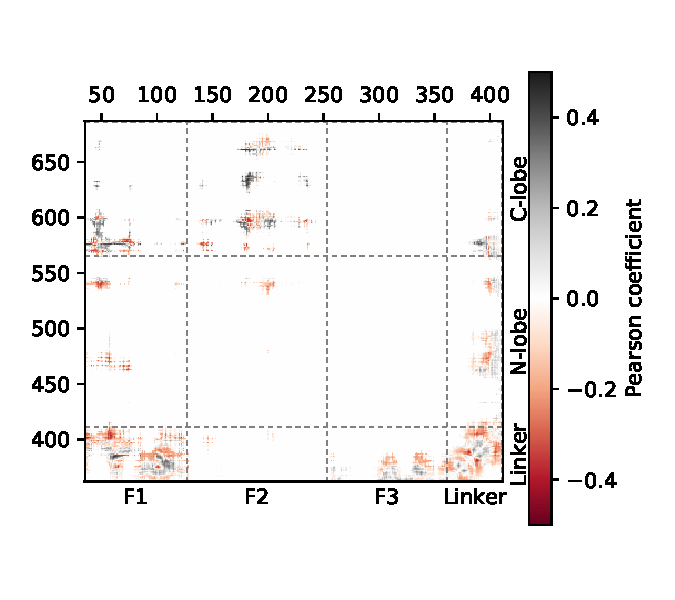
\includegraphics[width=.7\textwidth]{figures/results/interface_corr}
	\nicecaption{Correlations in contact map}{The contact map shows residue pairs, whose distance correlates with the applied force. The obtained slope is about $20\,\si{\pico\newton/\nano\metre}$.}
	\label{force:contactmap}
\end{figure}
%
%
%